% -*- mode Latex; -*-
\documentclass[a4paper]{report}
\usepackage{amsmath}
\usepackage{graphicx}
\usepackage[T1]{fontenc}
\usepackage{pslatex}
% \usepackage{palatino}
% \usepackage{ae,aecompl}
\begin{document}
\title{Manual for the use of Regress Pro Ellipsometry}
\author{F. Abbate}
\maketitle
\chapter{Introduction}
Regress Pro is a software to perform analysis of spectropic
ellipsometers of reflectometers. In this manual we will suppose that
you are familiar with the basic concepts of ellipsometry.

With Regress Pro you can define a model to describe the film stack and
you can also model each film layer to descibe its optical
properties. You will be also able to define a fit strategy well suited
to the problem under analysis.

With Regress Pro you will be able to determine the optical properties
of unknown materials or, if you already know the materials, you can
run simple fits to determine the thicknesses of the involved layers.

To characterize the optical properties of the materials Regress Pro
offers different optical models
\begin{itemize}
  \item Cauchy model
  \item Harmonic Oscillators model
  \item Lookup model
\end{itemize}
We will mention also that the EMA models are still not supported by
Regress Pro. The support for these models will be added, if possible,
in one of the next release of the software.

\chapter{Script Definition}
The first step to start to use Regress Pro is to define a film
stack. This can be done by describing the film stack in the ``Script''
tab. The best thing you can do is to start with one of the example
script provided with Regress Pro.
\begin{figure}[!thp]
  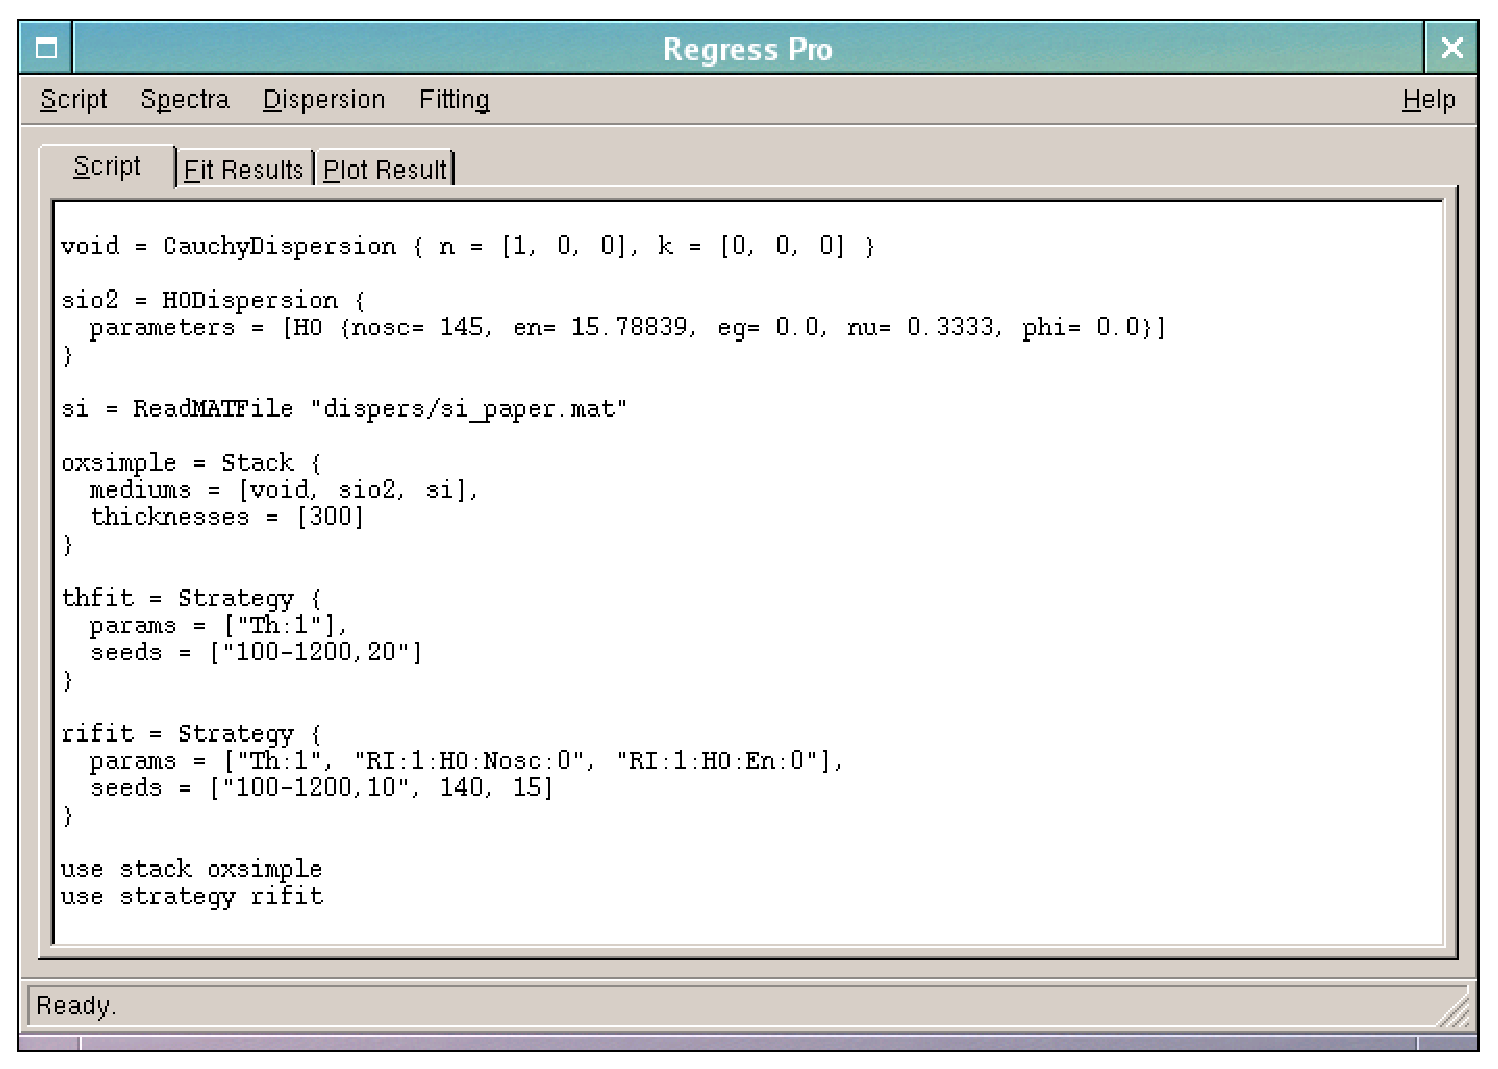
\includegraphics[width=\textwidth]{figure/script-window.eps}
  \caption{Script example with Regress Pro}
\end{figure}

\section{Film Stack description}
Before defining the film stack you have to define each of the involved
materials. Let's suppose that you want to define a simple oxide on
silicon film stack. Then you declare the material in the following way

\begin{verbatim}
void = Library "vacuum"
sio2 = Library "sio2"
si   = Library "si"
\end{verbatim}

What we have done is to load some pre-defined dispersion model from the library using the ``Library'' function.
This latter takes just a string as argument, it does perform a lookup in the library and return the appropriate model if it was found.

You can also load a dispersion table from a file.
Regress Pro accept files in the format ``.nk'' and ``.mat''.
These are two simple human-readable format that just gives the n and k (refractive index and absorption coefficient) at some sampling values of wavelength.
To load NK or MAT fil you can use the following instructions:

\begin{verbatim}
  sio2 = ReadNKFile "dispers/thermal-sio2.nk"

  si = ReadMATFile "dispers/si_paper.mat"
\end{verbatim}

If we use a table model for the oxide (sio2) you will not be able to fit any parameter because the values of n and k are fixed.
In this case we can do something more interesting and describe the oxide with an harmonic oscillators model.
In this case our definition will look like
\begin{verbatim}
sio2 = HODispersion {
  parameters = [HO {nosc= 145, en= 15.78839, eg= 0.0, nu= 0.3333, phi= 0.0}]
}
\end{verbatim}

The definition is quite self-explanatory. We are using the
``HODispersion'' tag to define an Harmonic Oscillator model. Then in
the field ``parameters'' we define all the parameters of the harmonicl
oscillators. The use of the square backet '[' means that here we can
provide, potentially, a list of comma separated values. In particular,
in this case, we can write in the list one term for each of the
harmonic oscillator that we want to use in the model. In this case we
have just one harmonic oscillator. Then, for each oscillator, we
provide 5 parameters:
\begin{itemize}
  \item nosc, Number of Oscillators for $\textrm{cm}^3$
  \item en, The Energy of the Oscillator, expessed in eV
  \item eg, The Absorption Bandwidth of the oscillator, expressed in
  eV
  \item nu, the Local Field Effect coefficient, normally you can keep
  it to the value of 1/3
  \item phi, the Phase of the Oscillator term, useful to describe
  absorbing peak in the DUV region
\end{itemize}
In this case we can keep ``eg'' and ``phi'' at 0 since the silicon
oxide is a non-absorbing dielectric.

Another possible model for the oxide is the Cauchy model.
Here an example where we define the dispersion model of an oxise using the Cauchy model:
\begin{verbatim}
sio2 = CauchyDispersion { 
  n = [1.45, 3.17e+03, 0], 
  k = [0,0,0]
}
\end{verbatim}

The definition of the Cauchy model can be found in the chapter about dispersion models.

Once we have defined all the materials we can easily describe the film
stack as follows
\begin{verbatim}
oxsimple = Stack {
  mediums = [void, sio2, si],
  thicknesses = [300]
}
\end{verbatim}

Even in this case the definition is quite self-explanatory. We have
defined a film stack, that we call ``oxsimple'', by using the tag
``Stack''. Then we define
\begin{itemize}
  \item the list of the mediums (materials composing the film stack)
  \item the default thicknesses for each layer
\end{itemize}
The definition of the mediums begin from the top and it ends with the
substrate at the bottom. In this case we have the sequence void, sio2
and si. Note that all the materials referenced here has been defined
previously in the script. In the ``thicknesses'' we provide just one
value, which is the thickness of the oxide layer. Note that this is a
default value and it can be changed if we decide to fit this
parameters.

\section{Fit Strategy Definition}
The next step after the definition of the film stack is to define the
fit strategy. It will define which parameters will be fitted, the seed
values and, in case, an uniformily spaced grid to search the best fit
value for a given parameters. Before to explain in detail the fit
strategy concept lets continue the previous example by defining a fit
strategy. It we want to fit only the thickness of the oxide we can
define something like that
\begin{verbatim}
thfit = Strategy {
  params = ["Th:1"],
  seeds = ["100-1200,20"]
}
\end{verbatim}
You can note that the tag to define a strategy is ``Strategy''. In
this case we have called our strategy ``thfit''. In the field
``params'' we will give a list of all the parameter that we want to
fit. We will provide later a detailed specification to describe all
the possible fit parameters. In the mean time, let's say that ``Th:1''
is the thickness of the layer 1. In Regress Pro the layer are numbered
from the top to the bottom. The layer 1 being the top most film layer
of the stack. Then we have defined the ``seeds'' field. This latter
gives the seed value for each of the parameters defined in
``params''. A seeds can be of two different type
\begin{itemize}
  \item a simple seed, just a number to be used as seed value
  \item a range specification of the form ``a-b,delta'' where a, b and
  delta are, respectively, the minimum, the maximum and the stride of
  the search grid, expressed in nm
\end{itemize}
As a matter of fact, if there is at least one parameters which gives
the seed specification if the form of a range, then a grid search will
be effectuated before starting the actual fit. The grid search is
useful because the fit algorithm is able to converge only if the seed
value is near enough to the solution. This is especially true for fit
of ellipsometric data because the model is strongly not-linear in its
parameters.

Let us provide, for the given example, another possible strategy that
we can define. This latter will be a fit strategy to determine both
the thickness and the refractive index of the oxide. It will look like
\begin{verbatim}
  rifit = Strategy {
  params = ["Th:1", "RI:1:HO:Nosc:0", "RI:1:HO:En:0"],
  seeds = ["100-1200,10", 140, 15]
}
\end{verbatim}
You can note that we have used a different name for differetiate this
strategy from the strategy defined before. If you look at the list of
the fit parameters you will see that the fist one is always the
thickness and we have added to more fit parameters to vary the
``Nosc'' and ``En'' paramter of the oxide. Note that this will work
correctly only if the oxide was defined with an harmonic oscillators
model. We will give a detailed explanation about the format of the fit
parameters laters. You can note that, for the two latter fit
parameters, we have provide a simple seed, without any range
specification. This is fine since we expect that, for un oxide like
material, the actual values of these parameters will be not far from
those of a thermal oxide.

A script will always terminate with some ``use'' directives like these
\begin{verbatim}
  use stack oxsimple
  use strategy thfit
\end{verbatim}
The directives are needed to specify which stack and which fit
strategy should be used because several film stack and fit strategies
can be defined within a single script.

\subsection{Fit Parameter Format}
The fit parameters are specified with a string. It will be in the
format ``Th:n'', where ``n'' is an integer, to specify the thickness of
the layer n. If you want to specify a fit parameter for the dispersion
model of one of the fit layers you should use the format
``RI:n:MODEL'', where n is still the layer number and MODEL is a
string that depends from the model which is actually used for the
film. For example, if the model is an harmonic oscillator it can be
the string ``HO:Nosc:i'', where HO specify that we expect an harmonic
oscillator model, ``Nosc'' indicates the parameter ``number of
oscillators'' and ``i'' is an integer that individuate the oscillator,
since a model can employ several different oscillators.

\subsection{The Grid strategy}
The grid strategy can be used when a given parameter should be
determined over a big range of variation. In this case you cannot
limit yourself to provide a seed value because the fit will not
converge. Regress Pro allows to use ``grid search'' approach that will
permit to explor a big window of variation for some (or all) of the
fit parameters. The grid will be used automatically if you define at
least one parameter in the form ``min-max,delta''. Please be careful
when you specify a grid search over several parameters because,
depending on the stride of each parameter, the grid search can be very
time consuming.

The general concept of the grid search is the following. All the
points defined by the grid will be tested and the corresponding
$\chi^2$ is evaluated. If the $\chi^2$ is less then a given thresold
(determined with the \textbf{set chisq\_thresold} directive) the point
is considered a good starting point. Then the point is used as a seed
to start the real fit. If you do not specify the thresold value for
the $\chi^2$ a predefined value will be used depending on the nature
of the spectrum that is loaded.

\subsection{``Use'' Directives}
The use directives allows to configure some global parameters of the
fit like ``max\_iterations'', ``chisq\_thresold'', ``range'' and
``subsampling''. The parameter ``chisq\_thresold'', in particular, is
useful because it determines when a point evaluated during the grid
search should be considered good enough to start the actual fit.

\chapter{Dispersion Models}

In this chapter we describe the different dispersions model available in Regress Pro.
Dispersion models are useful to describe the refractive index and the absorption coefficient of a material as a function of the wavelength.
Each kind of dispersion model can have different parameters that determines the behaviour of the refractive index with the wavelength.
When performing a fit of the experimental data the parameters of the dispersion model can be kept fixed or they can be given to the fit procedure to find the values of best fit.

\section{Harmonic Oscillator Model}
The Harmonic Oscillator model can be defined in the following form:
\begin{verbatim}
HODispersion {
  parameters = [
    HO {nosc= 145, en= 15.78, eg= 0.0, nu= 0.3333, phi=  0.0},
    HO {nosc= 10,  en= 6.5,   eg= 0.1, nu= 0.3333, phi= -0.7}]
}
\end{verbatim}
Each harmonic oscillator is identified by the tag ``HO'' with the parameters enclosed with braces.
You can define as many oscillator has you want but tipical model will have one up to six oscillator.

The mathematical definition of the harmonic oscillator is given by:
\begin{equation}
  \epsilon = 1 + \frac{\sum_i H_i}{1 - \sum_i \nu_i H_i}
\end{equation}
where $\epsilon$ is the dielectric constant.
The terms $H_i$ are the contributions of each harmonic oscillator and its defined by the following equation:
\begin{equation}
  H_i = A \frac{N_i \, e^{i \Phi_i}}{E_{n,i}^2 - E^2 + i E_{g,i} E}
\end{equation}
where $N_i$, $E_{n,i}$, $E_{g,i}$ and $\Phi_i$ are the parameters of the i-th harmonic oscillator, respectively Nosc, En, Eg and Phi.
The parameter $\nu_i$ takes into account the local field effect and is usually fixed to the theoretical value of $1/3$.
The constant $A$ is a normalization value fixed to 1.3732.

For the fit stategy the parameter of the HO model can be expressend in the form Nosc:i, En:i, Eg:i, Phi:i where i is a value that identifies the harmonic oscillator starting form zero for the first one.

You can therefore designate a complete parameter name using something like ``RI:2:HO:Nosc:0'' or ``RI:2:HO:En:1''.

\section{Cauchy Model}

The Cauchy model defines a refractive index that varies with the wavelength accordingly to the following equation:
\begin{equation}
  n = n_0 + \frac{n_1}{\lambda^2} + \frac{n_2}{\lambda^4}
\end{equation}
The coefficients $n_0$, $n_1$ and $n_2$ are expressed in $\textrm{nm}$ so that $n_1$ is in $\textrm{nm}^2$ and $n_2$ is in $\textrm{nm}^4$ while $n_0$ is adimensional.
For the k the same mathematical law is used even if, strictly speaking, the Cauchy model is for a non-absorbing dielectric wirh $k = 0$ in all the spectral range.

A Cauchy model can be declared in the following form:
\begin{verbatim}
sio2 = CauchyDispersion { 
  n = [1.45, 3.17e+03, 0], 
  k = [0,0,0]
}
\end{verbatim}
The coefficients ``n'' are given in the order $n_0$, $n_1$ and $n_2$. The field ``k'', similarly, describes the coefficient $k_0$, $k_1$ and $k_2$ in the given order.

When defining a fit strategy you can refer to the Cauchy coefficients ``n'' as ``N0'', ``N1'' and ``N2''. For the coefficients ``k'' the logic is the same and the parameters are named ``K0'', ``K1'' and ``K2''.

You can therefore designate a complete parameter name using something like ``RI:2:Cauchy:N0''.

\section{Lookup Model}

The lookup model can be used whenever the material can have different refractive index depending on a single numeric parameter.
Usually the parameter is related to a physical or chemical property of the film so that the value of the parameter is directly related to the state of the material.
A tipical example is a material that incorporate a percentage of a different atomic element.
In such case you can assume that for each atomic percentage the material will have a specific refractive index that varies regularly with the parameter itself.

The main idea behind the lookup model is that you identify a single physical parameter that determine the optical properties of the film.
Then you should identify a range of variability of such parameter.
In the interval of variation of the parameter you should identify some values for which you provide a known curve of refractive index.
In this way, when you use the lookup model, the refractive index can be calculated for any value of the parameter by using a linear interpolation of the closest samples available.

To make everything more clear let us suppose that we have a SiGe film that is produced under controlled conditions.
Let us assume that the only parameter that determine the optical properties of the film is the atomic percentage of the Ge.
In this case we can choose the Ge\% as a parameter for the lookup model.
Then we can provide the dispersion curves of n and k for some given values of Ge\%.
Let us suppose, for example, that we know the curve at Ge = 0\%, 5\%, 10\%, and 15\%.
In this case we can define a lookup model with a parameter that can goes from 0 up to 15 to cover all the known interval.
Then if we cant to know the n and k at Ge = 7\% the values will be calculated by linear interpolation from the closest sample at 5\% and 10\%.

The lookup model can be described as follows:
\begin{verbatim}
sige = LookupDispersion { 
  name = "Pseudo-amorphe SiGe",
  values = [0, 5, 10, 15],
  dispersions = [sige0, sige5, sige10, sige15],
  predef = 8.5
}
\end{verbatim}
using the fields ``values'' and ``dispersions'' we define, in the order, the sampling values of the parameter and the corresponding dispersion curves.
In the example above we assume that we have previously defined ``sige0'', ``sige5'', etc and that they corresponds to the dispersion curve of SiGe for the Ge\% at 0, 5, 10\% etc.
The field ``predef'' declares what should be the default value of the parameters and is a mandatory field.

When you define a fit strategy you can refer to the parameter of the lookup model by just using the letter ``P''.
So, for example, the complete name of the parameter could be something like ``RI:2:Lookup:P''.

\chapter{Multiple Fit}

In some cases you can have multiple experimental acquisition of spectra caming from samples prepared under different conditions.
If all these samples can be modelized using the same film stack you can take advantage of the ``Multiple Fit'' function offered by Regress Pro.
The multiple fit let you load several samples to perform a simultaneous fit af all of them.

When performing a simultaneous fit you can have two category of fitting parameters, that is:
\begin{itemize}
  \item common parameters
  \item individual sample's parameters.
\end{itemize}
The difference is that common parameters are applied with the same value to all the samples while individual parameters are specific of each sample.

The multiple fit function is particularly useful in same cases when a simple fit could led to a systematic error in the determination of some of the fitting parameters.
In this case you can use a multiple fit with same samples prepared under different condition in order to eliminate or greatly reduce the systematic errors.
The reason why it works is that the algorithm have more indipendent data (experimental spectra) to check the proposed value of the fit parameters reducing therefore the possibility of ``false solutions''.

In order to use the multiple fit feature you should prepare a specific script that provides some additional informations about the samples.

Let us give an example to illustrate more easily how it works. First we define our materials and film stack as usually:
\begin{verbatim}
si   = Library "si"
sio2 = Library "sio2"
void = Library "vacuum"

sin = HODispersion {
  name = "SiN",
  parameters = [
    HO {nosc= 74.3444, en= 8.35617, eg= 0.474468, nu= 0.3333, phi=-0.0120003}]
}

dti= Stack {
  mediums = [void, sio2, sin, sio2, si],
  thicknesses = [423, 91, 7.5]
  }
\end{verbatim}
Once we have defined the film stack we can proceed to define the sample specific informations. Here an example:

\begin{verbatim}

sample00 = Sample {
  spectrum = "examples/multi-fit/samples/test2787.dat",
  constraints = [],
  individual = [328, 89]

}

sample01 = Sample {
  spectrum = "examples/multi-fit/samples/test2771.dat",
  constraints = [],
  individual = [422, 89]

}

sample02 = Sample {
  spectrum = "examples/multi-fit/samples/test2783.dat",
  constraints = [],
  individual = [291, 89]

}

sample03 = Sample {
  spectrum = "examples/multi-fit/samples/test2784.dat",
  constraints = [],
  individual = [353, 89]

}

rifit = Strategy {
  params = [ "RI:2:HO:Nosc:0", "RI:2:HO:En:0", "RI:2:HO:Eg:0",
             "RI:2:HO:Phi:0" ],
  seeds = [ 74, 8, 0.4, 0]
}

mfit = MultiFit {
  samples = [sample00, sample01, sample02, sample03],
  contraints = [],
  individual = [ "Th:1", "Th:2" ]    
}
\end{verbatim}

In order to better understand let as look first at the end of the snippet above wheres we define an object of type \texttt{MultiFit}. This object is very important for the multiple fit and it does defines:
\begin{itemize}
  \item the list of samples to be used
  \item the list of the constraint parameters
  \item the list of the individual parameters
\end{itemize}

The constraints are parameters that you can set to some specific values for each sample.
Then you give the list of the individual parameters.
These latter will be fitted by the algorithm by using a different value for each sample.

You may also note that we did not define the list of the common parameters.
The reason is very simple, the common parameters are those defined in the \texttt{Strategy} as you do normally for a simple fit.
The common parameters are common to all the samples and their values are applied to all the samples by the fitting algorithm.

Now we can go back to the definition of the ``samples''. As you can see we define multiple \texttt{samples} to describe all the experimental samples that we want to use.
For each sample we give the values of the constraints and the seed values of the individual parameters.
The list for the constraints and individual parameters should be simple list of numbers and their lengths should match the number of parameters or constraints that you have declared in the \texttt{MultipleFit} object.

So the complete definition of the \texttt{Sample} includes:
\begin{itemize}
  \item \texttt{spectrum}, the spectrum file to be loaded
  \item \texttt{constraints}, the value of the parameters setted to a fixed different value for each sample
  \item \texttt{individual}, the seed value to be used for the sample's individual parameters
\end{itemize}

At this point we can just terminate the script as follow:
\begin{verbatim}
set max_iterations 200

use stack dti
use strategy rifit
use multi_fit mfit
\end{verbatim}

You can see that it is just like a simple fit with the only difference that we have declared the multiple fit object that should be used.
The declaration is for the case you may have defined several multiple fit objects in the script.
In this case you just specify which one to use by using the \texttt{use} directive.

Once you have defined the script strategy the most difficult part of the work is done.
Now you have just to choose \textsf{Fitting $\rightarrow$ Run Multiple Fit} from the menu to start the fitting of the data.

Please note that the multiple fit will *not* produce any plot but the results will be shown in the ``Fit Results'' sheet.
You will find the values obtained for the common and individual parameters and the residual $\chi^2$ for each sample.
It is very important to verify the residual $\chi^2$ of each sample to be sure that nothing went wrong during the multiple fit.

\chapter{Running a Fit}
To actual running a fit you have to
\begin{enumerate}
  \item define or load a script
  \item load a spectrum.
\end{enumerate}
To load a spectrum you can use the function of the menu. The spectrum
should be in a format specific of Regress Pro. This format is in ASCII
format and is very easy to understand. You can just look to the
examples provided with Regress Pro to understand how the data should
be formatted.

Once you have loaded a spectrum you can start the fitting by using the
function of the menu ``\textsf{Fitting $\rightarrow$ Run Fitting}''. If the
fitting has been successful the results will be presented in the tabs
``Fit results'' and ``Plot results''. In ``Fit results'' you will find
the results of the fit plus some informations, more or less
useful. Then in the ``Plot results'' tab you will find a plot with the
experimental spectrum and the model. The golden rule of spectroscopic
ellipsometry is that \emph{a fit is good if the model corresponds to
the experimental spectrum}.

In the figure you will find un example of a successful fit.
\begin{figure}[!thp]
  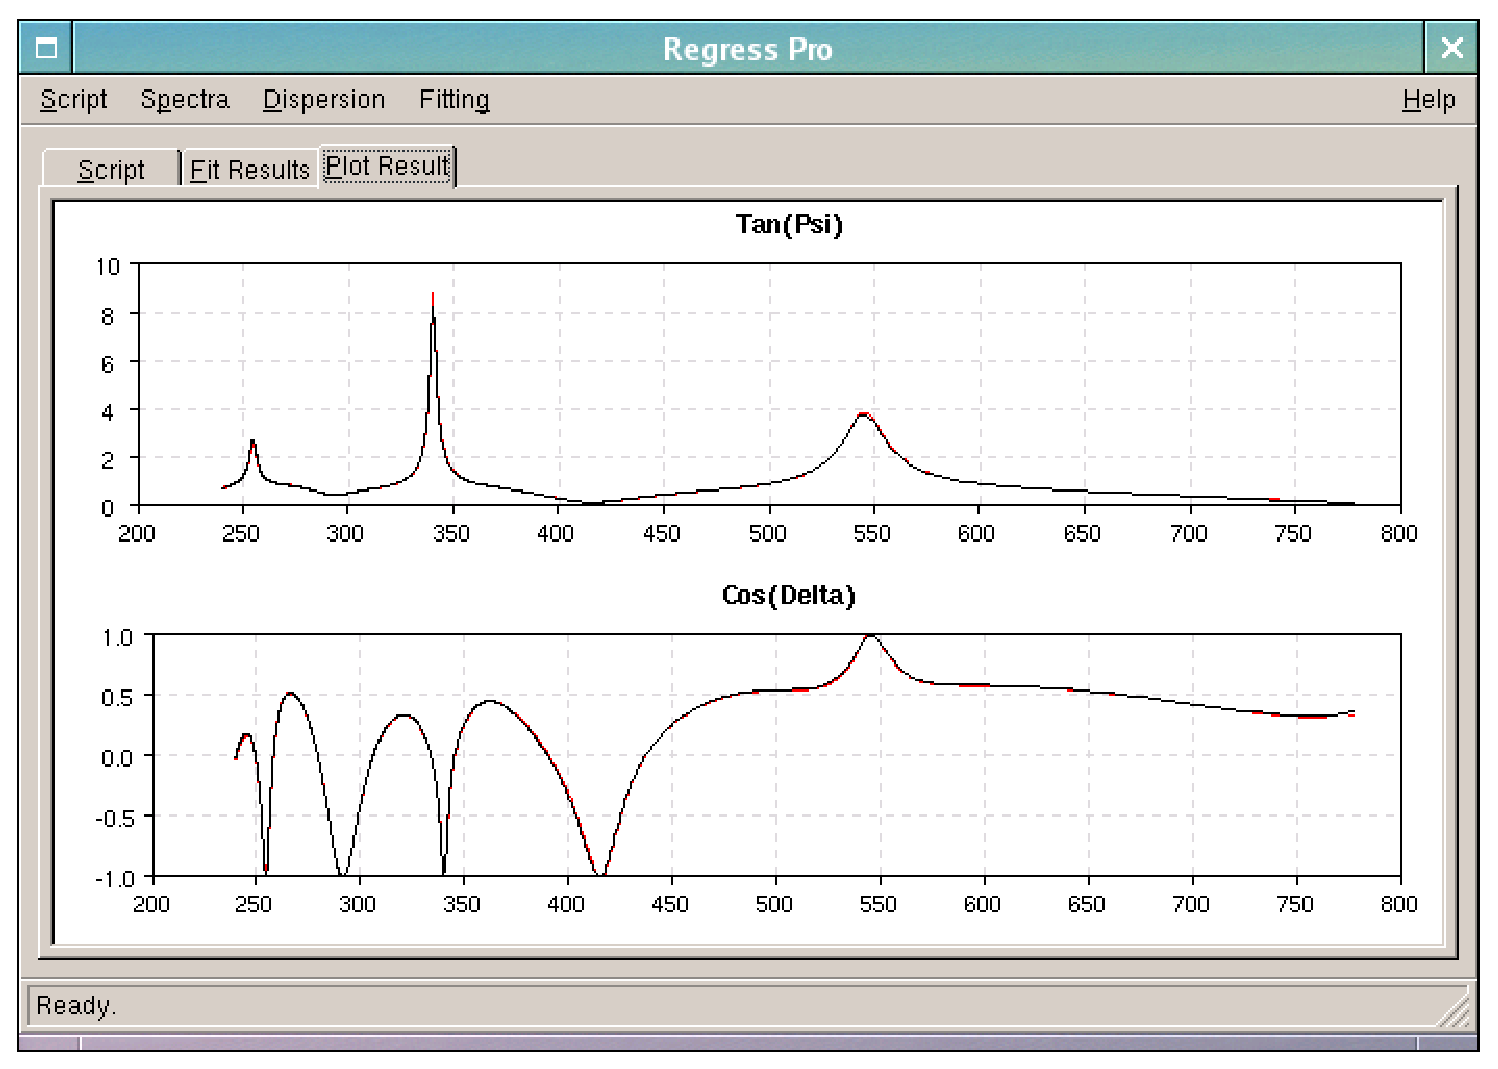
\includegraphics[width=\textwidth]{figure/oxide-fit-1.eps}
  \caption{Fit of a ellipsometric fit of a silicon oxide}
\end{figure}

\end{document}
